\subsubsubsection{Probing the Higgs boson self-coupling in di-Higgs
  production with full $m_t$-dependence at NLO QCD}
\label{subsec:varylambda}

\begin{center}
\textit{by  Gudrun Heinrich, Stephen Jones, Matthias Kerner, Gionata Luisoni, Ludovic Scyboz}
\end{center}

%While the couplings of the Higgs boson to vector bosons are very well measured meanwhile, and the couplings to third generation fermions also start to be well constrained and seem to confirm the Standard Model, the Higgs boson self-coupling could still reveal clear signs of New Physics. As it is not too far-fetched to have BSM scenarios in mind where the trilinear Higgs boson coupling $\lambda$ is different from the SM value at the ${\cal O}(10\%)$ level, while the deviations in other Higgs boson couplings are at the percent level, we consider $\lambda$ variations only in this section.
In this section we consider the impact of varying the Higgs self-coupling $\lambda$ on the NLO computations of the HH production cross section.
In particular, we announce a version of the {\tt ggHH} code~\cite{Borowka:2016ypz,Heinrich:2017kxx,Borowka:2016ehy} implemented in the {\tt POWHEG-BOX-V2}~\cite{Alioli:2010xd} where variations of  $\lambda$ are accessible to the user in a parton shower Monte Carlo program at full NLO.

\subsubsubsection{Total cross sections at different values of the trilinear coupling}

In Table \ref{tab:sigmatot} we list total cross sections at 14\,\UTeV and 27\,\UTeV for various values of the trilinear Higgs coupling $\lambda$. 
\begin{table}[htb]
\begin{center}
%\setlength{\extrarowheight}{3.0pt}
\begin{tabular}{| c | c | c |c|c|}
%\Xhline{2\arrayrulewidth}
\hline
&&&&\\
$\lambda_{\mathrm{BSM}}/\lambda_{\mathrm{SM}}$ & $\sigma_{\rm{NLO}}@14 \mathrm{\UTeV}$\,[fb] & $\sigma_{\rm{NLO}}@27 \mathrm{\UTeV}$\,[fb] &K-fac.@14TeV&K-fac.@27TeV\\
&&&&\\
\hline
1& 32.88$^{+13.5\%}_{-12.5\%}$&127.7$^{+11.5\%}_{-10.4\%}$ &1.66&1.62\\
\hline
2 & 14.91 &  59.10 & 1.58 & 1.52\\
\hline
2.4 & 13.81& 53.67 & 1.65 & 1.60\\
\hline
3& 19.82 & 69.84 & 1.97 & 1.89\\
\hline 
5 & 98.42& 330.61 & 2.21 & 2.18\\
\hline 
0 & 73.84& 275.29& 1.79 & 1.78 \\
\hline 
-1 & 137.69& 504.9 & 1.87 & 1.83\\
\hline
%\Xhline{2\arrayrulewidth}
\end{tabular}
\end{center}
\caption{Total cross sections for Higgs boson pair production at full NLO. The given uncertainties are scale uncertainties. 
\label{tab:sigmatot}}
\end{table}

The results have been obtained using the parton distribution functions PDF4LHC15\_nlo\_100\_pdfas~\cite{Butterworth:2015oua,CT14,MMHT14,Ball:2014uwa},
along with the corresponding value for $\alpha_s$ for both the NLO and
the LO calculation.
The masses have been set to $m_h=125$\,\UGeV, $m_t=173$\,\UGeV,
and the top quark width has been set to zero. 
The scale uncertainties are the result of a 7-point scale variation around the central scale $\mu_0 = m_{hh}/2$,
with $\mu_{R,F}=c_{R,F}\,\mu_0$, where 
$c_R,c_F\in \{2,1,0.5\}$, except that the extreme variations $(c_R,c_F)=(2,0.5)$ and $(c_R,c_F)=(0.5,2)$
are omitted. 

Table~\ref{tab:sigmatot} also shows that the K-factors do vary substantially as functions of the trilinear coupling.
This fact is illustrated in Fig.~\ref{fig:Kfacvariation}, where it is demonstrated that the K-factor takes values between 1.57 and 2.16
%if the trilinear coupling is varied between $-5\leq \chhh\leq 12$.

\begin{figure}[htb]
  \centering
    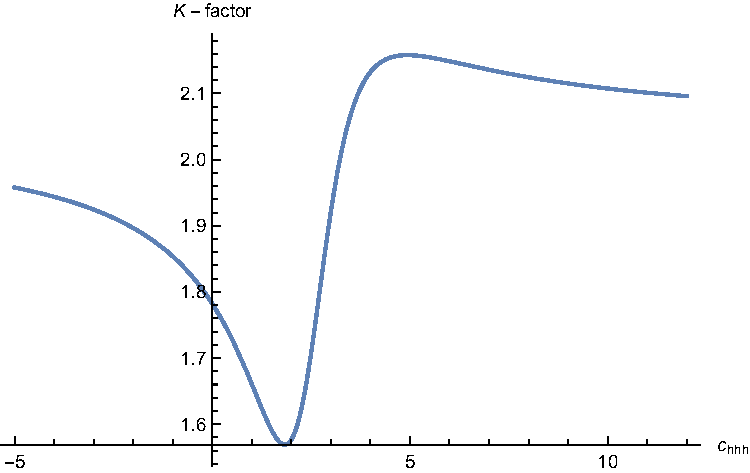
\includegraphics[width=0.4\textwidth]{\main/section3/plots/Kfac_varlambda.pdf}
%  \includegraphics[width=\textwidth]{plots/}
%    \caption{\label{fig:lambda_large_27}}
\caption{Variation of the NLO K-factor with the trilinear coupling, $\sqrt{s}=14$\,\UTeV.}
\label{fig:Kfacvariation}
\end{figure}


\subsubsubsection{Differential cross sections  at 14 \UTeV and 27 \UTeV}

In Figs.~\ref{fig:lambda_small} and ~\ref{fig:lambda_large} we show the $\mhh$ distribution for various values of $\lambda=\lambda_{\mathrm{BSM}}/\lambda_{\mathrm{SM}}$ at 14 \UTeV.
Figs.~\ref{fig:lambda_small_27} and ~\ref{fig:lambda_large_27} 
 show results for the $\mhh$ distribution at 27 \UTeV. The scale variation band for $\lambda=1$ is also included.
 Note that $\lambda=2.4$ is the value where the cross section as a function of $\lambda$ goes through a minimum, due to maximal destructive interference between diagrams containing the trilinear coupling and diagrams which do not contain Higgs boson self-couplings.
 
\begin{figure}[htb]
  \centering
  \subfloat[]{\label{fig:lambda_small_14}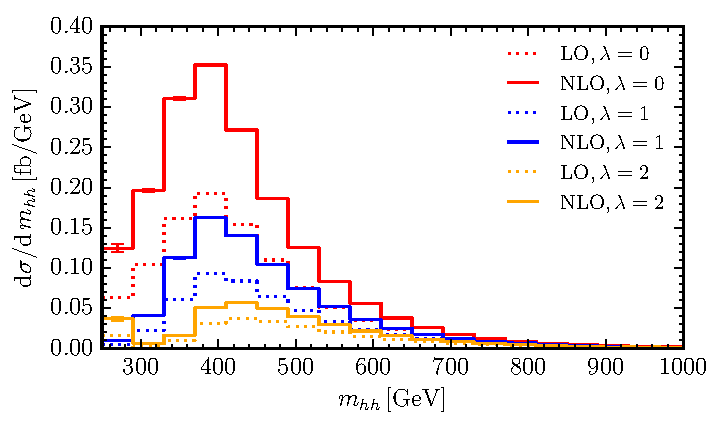
\includegraphics[width=0.6\textwidth]{\main/section3/plots/mhh_Kfac_14TeV_varylambda_small.pdf}}
  %\hfill
  %\subfloat[]{\label{fig:lambda_small_27}}
  %  \includegraphics[width=\textwidth]{plots/}
 \caption{Higgs boson pair invariant mass distributions for various values of $\lambda$ (relative to $\lambda_{\mathrm{SM}}$)  at 14\,\UTeV.}
\label{fig:lambda_small}
\end{figure}
%
\begin{figure}[htb]
  \centering
    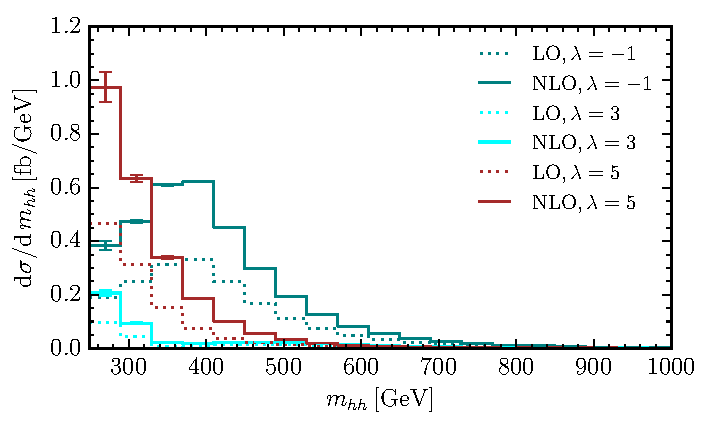
\includegraphics[width=0.6\textwidth]{\main/section3/plots/mhh_Kfac_14TeV_varylambda_large.pdf}
%  \includegraphics[width=\textwidth]{plots/}
%    \caption{\label{fig:lambda_large_27}}
\caption{Higgs boson pair invariant mass distributions for $\lambda=\lambda_{\mathrm{BSM}}/\lambda_{\mathrm{SM}}=-1,3,5$  at 14\,\UTeV.}
\label{fig:lambda_large}
\end{figure}

\begin{figure}[htb]
  \centering
    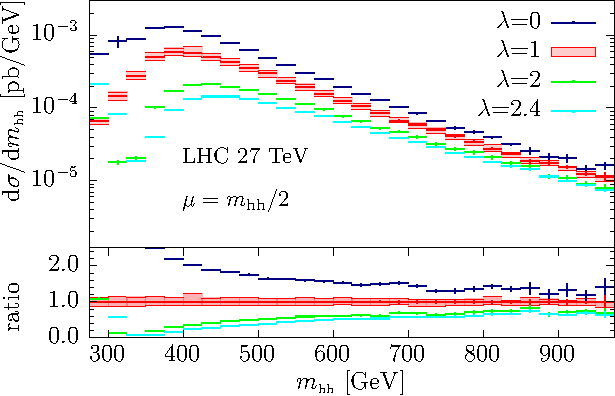
\includegraphics[width=0.6\textwidth]{\main/section3/plots/NLO_mHH_small_lambda_27TeV.pdf}
%  \includegraphics[width=\textwidth]{plots/}
%    \caption{\label{fig:lambda_large_27}}
\caption{Higgs boson pair invariant mass distributions for $\lambda=\lambda_{\mathrm{BSM}}/\lambda_{\mathrm{SM}}=0,1,2,2.4$  at 27\,\UTeV. The scale uncertainties for the SM value of $\chhh$ are shown as a red band.}
\label{fig:lambda_small_27}
\end{figure}

\begin{figure}[htb]
  \centering
    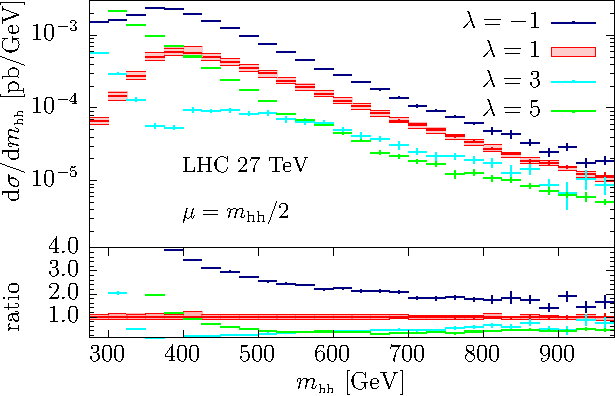
\includegraphics[width=0.6\textwidth]{\main/section3/plots/NLO_mHH_large_lambda_27TeV.pdf}
%  \includegraphics[width=\textwidth]{plots/}
%    \caption{\label{fig:lambda_large_27}}
\caption{Higgs boson pair invariant mass distributions for $\lambda=\lambda_{\mathrm{BSM}}/\lambda_{\mathrm{SM}}=-1,1,3,5$)  at 27\,\UTeV. The scale uncertainties for the SM value of $\lambda$ are shown as a red band.}
\label{fig:lambda_large_27}
\end{figure}

\begin{figure}[ht]
\begin{center}
  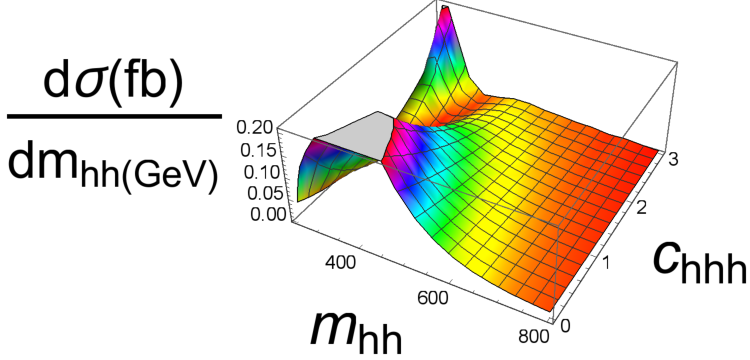
\includegraphics[width=0.45\textwidth]{\main/section3/plots/3D_mhh_chhh.pdf}    
\end{center}
\caption{3-dimensional visualisation of the $\mhh$ distribution at
  14\,\UTeV, as a function  $\lambda$.}
\label{fig:chhh_3D}
\end{figure}
Fig.~\ref{fig:chhh_3D} shows the Higgs boson pair invariant mass
distributions at NLO as a function of $\lambda=\chhh$  as a 3-dimensional heat map.
The dip in the distribution around $\chhh=2.4$ is clearly visible.
 
%\bibliography{bib/refs_HH_lambda}


